% This work is licensed under the Creative Commons
% Attribution-NonCommercial-ShareAlike 4.0 International License. To view a copy
% of this license, visit http://creativecommons.org/licenses/by-nc-sa/4.0/ or
% send a letter to Creative Commons, PO Box 1866, Mountain View, CA 94042, USA.

\chapter{Brownsche Bewegung} %10

\begin{defi}\ %nonumber
	\begin{itemize}
		\item Ein stochastischer Prozess in \textbf{stetiger Zeit} ist eine messbare Abbildung 
\begin{align*}
	X\colon[0,T]\times\Omega\to\R^d,\qquad(t,\omega)\mapsto X_t(\omega).
\end{align*}
		\item Wir nennen $X$ einen \textbf{stetigen stochastischen Prozess}, wenn alle Pfade bis auf Nullmengen stetig sind, d.h.
		\begin{align*}
		:\Longleftrightarrow t\mapsto X_t(\omega)\text{ ist stetig }\qquad\forall \omega\in\Omega\setminus A \mit A~\P\text{-Nullmenge}
		\end{align*}
	\end{itemize}
\end{defi}

Die \textit{Brownsche Bewegung} ist:
\begin{itemize}
	\item stetige Verallgemeinerung von Random Walks
	\item Klassisches Modell für "zufällige Bewegung" in $\R^d$.
	\item Zur Ideengeschichte: 
	\begin{itemize}
		\item Zitterbewegung von Blütenpollen auf Wasser (Robert Brown 1828)
		\item \textit{Brownsche Molekularbewegung} (Einstein, Smolochowski 1909)
		\item Finanzmathematik: Zufällige Preisbewegungen (Bachelier 1900)
		\item Norbert Wiener (1923): erste rigorose mathematische Beschreibung\\
		Deshalb heißt die Brownsche Bewegung oft auch \textbf{Wiener Prozess}.
	\end{itemize}		
\end{itemize}

\begin{defi}
	Ein reellwertiger stochastischer Prozess $B:=(B_t)_{t\in[0,T]}$ heißt\\ \textbf{(standardisierte) Brownsche Bewegung (BB)}, wenn:
	\begin{enumerate}[label=\alph*)]
		\item $\begin{aligned}
			B_0=0
		\end{aligned}$ (Standardisierung)
		\item $B$ hat \textbf{unabhängige Zuwächse}, d.h. für beliebige Zeitpunkte\\ $0\leq t_1<t_2<\ldots<t_N\leq T$ sind die Zufallsvariablen
		\begin{align*}
			\left(B_{t_1}-B_0\right),\left(B_{t_2}-B_{t_1}\right),\ldots,\left(B_{t_N}-B_{t_{N-1}}\right)
		\end{align*}
		unabhängig.
		\item $\begin{aligned}
			\big(B_t-B_s\big)\sim\Nor(0,t-s)\qquad\forall 0\leq s\leq t\leq T
		\end{aligned}$  (\textbf{stationäre, normalverteilte Zuwächse})
		\item $B$ ist ein stetiger stochastischer Prozess.
	\end{enumerate}
\end{defi}

Alternative Charakterisierung als Gaußscher Prozess:

\begin{defi}
	Ein stochastischer Prozess $(X_t)_{t\in[0,T]}$ heißt \textbf{Gaußscher Prozess}
	\begin{align*}
		:\Longleftrightarrow \Big(X_{t_1},X_{t_2},\ldots,X_{t_N}\Big)\text{ (multivariat) normalverteilt ist }\forall0\leq t_1\leq t_2\leq\ldots\leq t_n\leq T  
	\end{align*}
	Hierbei sind $\big(X_{t_1},X_{t_2},\ldots,X_{t_N}\big)$ die \textbf{endlich-dimensionalen Randverteilungen}.
\end{defi}

\begin{lemma}\label{10.1}
	Sei $(X_t)_{t\in [0,T]}$ ein stetiger Gaußscher Prozess mit 
	\begin{itemize}
		\item $\begin{aligned}
			X_0=0
		\end{aligned}$
		\item $\begin{aligned}
			\E\big[X_t]=0 \hspace{90pt}\forall t\in[0,T]
		\end{aligned}$
		\item $\begin{aligned}
			\Cov\big(X_t,X_s\big)=\min(s,t) \qquad\forall s,t\in[0,T]
		\end{aligned}$
	\end{itemize}
	Dann ist $X$ eine Brownsche Bewegung.
\end{lemma}

\begin{proof}
	Zu zeigen: unabhängige Zuwächse und $\Var\big(X_t-X_s\big)=t-s$.\\
	Sei $X$ Gaußscher Prozess. 
	Setze $Y:=\big(X_{t_1},\ldots,X_{t_N}\big)\sim$ multivariat Normalverteilt.
	\begin{align*}
		\left(X_{t_2}-X_{t_1},\ldots,X_{t_N}-X_{t_{N-1}}\right)
		&=\begin{pmatrix}
			-1 & 1 & 0 & 0 & \hdots & 0\\
			0 & -1 & 1 & 0 & \hdots & \vdots\\
			0 & 0 & -1 & 1 & \hdots & \vdots\\
			\vdots & \ddots & \ddots & \ddots & \vdots & 0\\
			0 & \hdots & \hdots & 0 & -1 & 1
		\end{pmatrix}\cdot Y
	\end{align*}
	ist wieder multivariat normalverteilt.\\
	D.h. die Zuwächse sind unkorreliert!
	Sei $i\leq j$.
	\begin{align*}
		&\Cov\left(X_{t_j}-X_{t_{j-1}},X_{t_i}-X_{t_{i-1}}\right)\\
		&=\E\left[\left(X_{t_j}-X_{t_{j-1}}\right)\cdot\left(X_{t_i}-X_{t_{i-1}}\right)\right]\\
		&=\E\big[X_{t_j}\cdot X_{t_i}\big]-\E\big[X_{t_{j-1}}\cdot X_{t_i}\big]-\E\big[X_{t_j}\cdot X_{t_{i-1}}\big]+\E\big[X_{t_{j-1}}\cdot X_{t_{i-1}}\big]\\
		&=\min\lbrace t_j,t_i\rbrace-\min\lbrace t_{j-1},t_i\rbrace-\min\lbrace t_j,t_{i-1}\rbrace+\min\lbrace t_{j-1},t_{i-1}\rbrace\\
		&=t_i-t_i+t_{i-1}+t_{i-1}\\
		&=0
	\end{align*}
	
	Also sind die Zuwächse von $X$ unabhängig.
	Zur Varianz:
	\begin{align*}
		\Var\big(X_t-X_s\big)
		&=\E\left[\big(X_t-X-s\big)^2\right]\\
		&=\E\left[X_t^2-2\cdot X_s\cdot (X_t-X_s)-X_s^2\right]\\
		&=\underbrace{\E\big[X_t^2\big]}_{=t}-2\cdot\E\Big[\underbrace{\big(X_s-X_0\big)\cdot\big(X_t-X_s\big)}_{\unab}\Big]-\underbrace{\E\big[X_s^2\big]}_{=s}\\
		&=t-s
	\end{align*}
\end{proof}

\subsection*{\textbf{Wavelet-Konstruktion} der BB auf $[0,1]$:}
Betrachte den Hilbertraum $L_2([0,1])$ mit ONB $(\psi_k)_{k\in\N}$. (Später Haar-Wavelets)
\begin{align*}
	&\text{Inneres Produkt:} &\langle f,g\rangle&=\int\limits_0^1 f(x)\cdot g(x)\d x\\
	&\text{Parselvalsche Ungleichung:} &\langle f,g\rangle&=\sum\limits_{k=0}^\infty\langle f,\psi_k\rangle\cdot\langle g,\psi_k\rangle
\end{align*}

\begin{theorem}\label{theorem10.2}
	Seien $(Z_k)_{k\in\N}$ iid Folge von standardnormalverteilten Zufallsvariablen. Setze
	\begin{align}\label{eqWaveletKonstruktionStern}\tag{$\ast$}
		B_t:=\sum\limits_{k=0}^\infty Z_k\cdot\int\limits_0^t\psi_k(s)\d s\qquad\forall t\in[0,1]
	\end{align}
	Behauptung: $B$ ist Brownsche Bewegung
\end{theorem}

Zu zeigen:
\begin{enumerate}[label=\alph*)]
	\item Summe konvergiert in $L_2(\d\P)$ für jedes $t\in[0,1]$. (Beachte $L_2([0,1])\neq L_2(\d\P)$)
	\item $\begin{aligned}
		\E\big[B_t\big]=0\text{ und }\Cov\big(B_t-B_s\big)=\min\lbrace s,t\rbrace
	\end{aligned}$
	\item $B$ ist Gaußscher Prozess
	\item Summe in \eqref{eqWaveletKonstruktionStern} konvergiert fast sicher gleichmäßig in $t$
	\begin{align*}
		\implies B\text{ ist stetiger Prozess.}
	\end{align*}
\end{enumerate}

Für $(\psi_k)_{k\in\N}$ verwenden wir die \textbf{Haar-Basis} $\big(h_k(s)\big)_{k\in\N}$: $h_0 = 1$

\begin{figure}[H]
	\begin{center}
		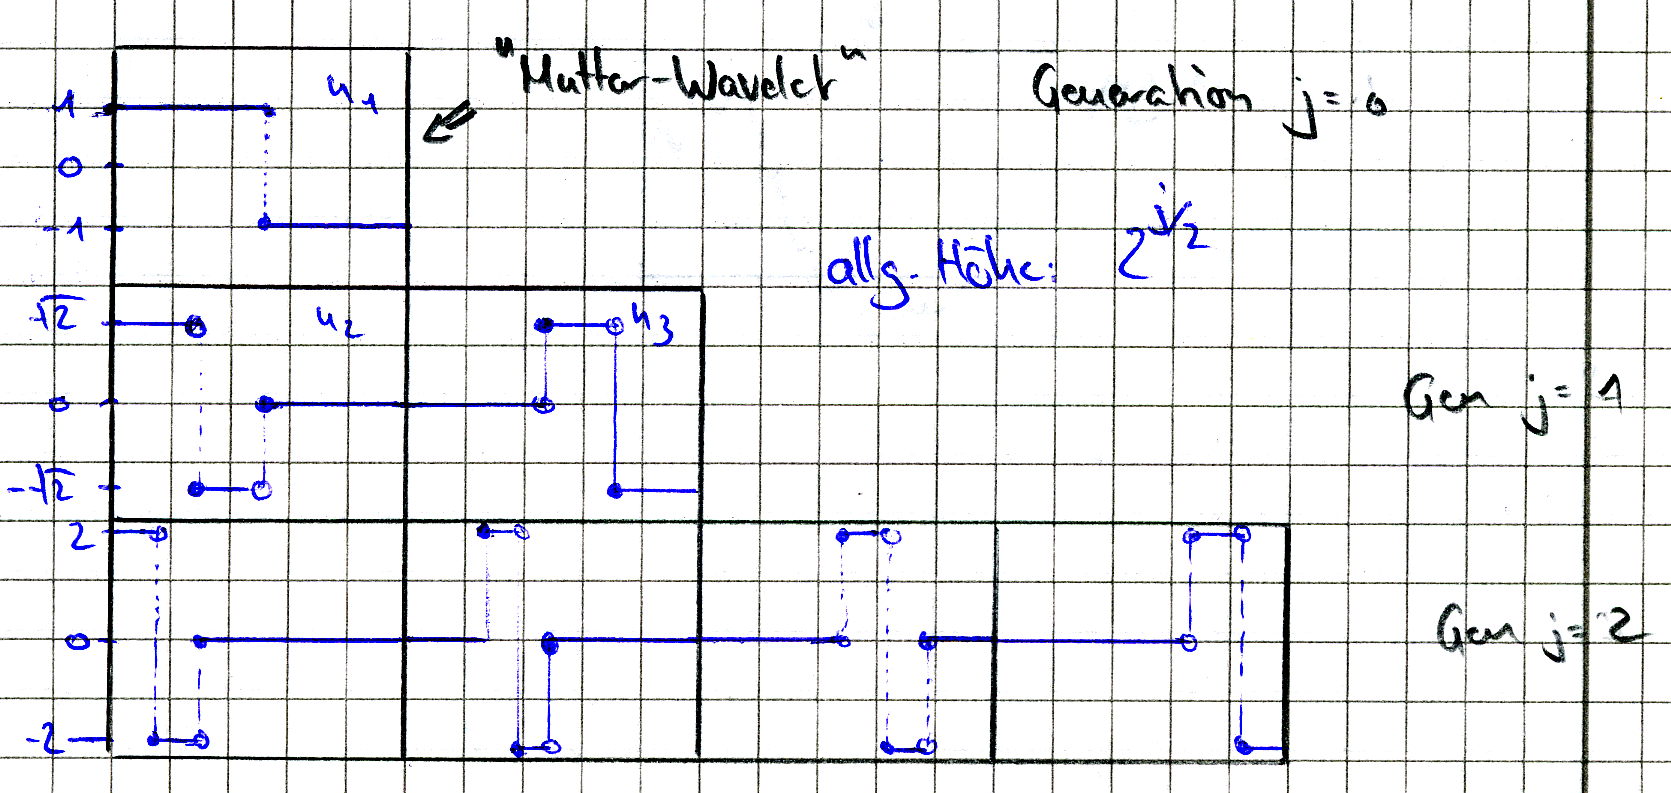
\includegraphics[width=1\textwidth]{./pics/WTHMscan001.png}
		\caption{Generation $j=0,1,2$ der Haar-Basis}
		\label{AbbHaarBasis}
	\end{center}
\end{figure}
Die allgemeine Höhe der Wavelets beträgt: $\frac{1}{2}\cdot2^{-\frac{j}{2}}$.
Jetzt integrieren wir die Wavelets aus Abbildung \ref{AbbHaarBasis} und erhalten die integierte Haar-Basis
\begin{align*}
	H_k(t):=\int\limits_0^t h_k(s)\d s
\end{align*}

\begin{figure}[H]
	\begin{center}
		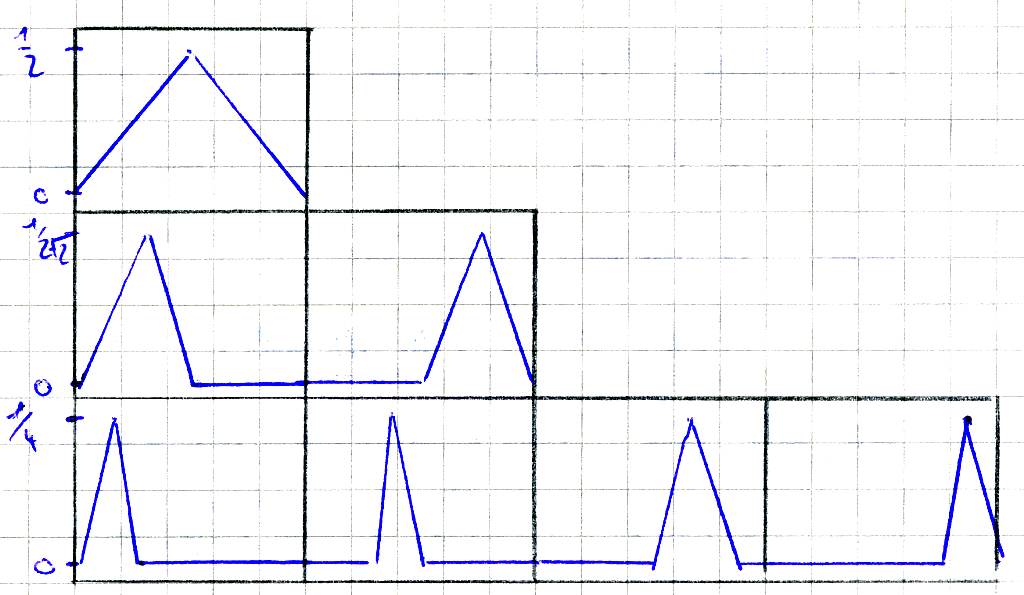
\includegraphics[width=1\textwidth]{./pics/WTHMscan002.png}
		\caption{Integrierte Wavelets}
		\label{AbbHaarIntegrierteWavelets}
	\end{center}
\end{figure}

Approximation der Brownschen Bewegung:
Es kommen also immer neue, zufällige Auslenkungen dazu.

\begin{figure}[H]
	\begin{center}
		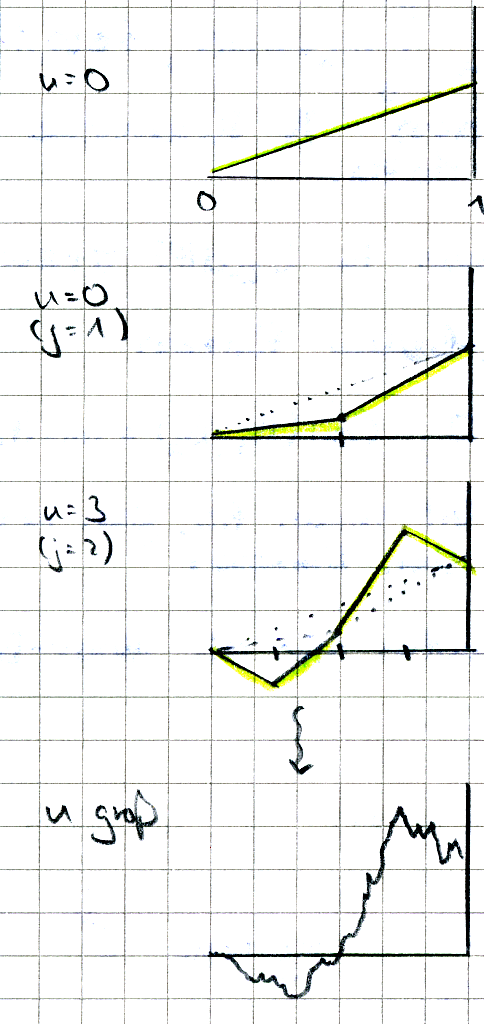
\includegraphics[width=0.5\textwidth]{./pics/WTHMscan003.png}
		\caption{Approximation der Brownschen Bewegung}
		\label{AbbBBn}
	\end{center}
\end{figure}

\begin{proof}
	Setze
	\begin{align*}
		B_t^N:=\sum\limits_{k=0}^N Z_k\cdot\int\limits_0^t h_k(s)\d s
	\end{align*}
	
	\underline{Zeige a):}
	Es gilt:
	\begin{align*}
		\big\Vert B_t^N-B_t^M\big\Vert_{L_2(\d\P)}^2
		&=\E\Big[\big(B_t^N-B_t^M\big)\Big]\\
		&=\E\left[\left(\sum\limits_{n=M+1}^N Z_n\cdot\int\limits_0^t h_n(s)\d s\right)^2\right]\\
		&=\sum\limits_{n=M+1}^N\sum\limits_{j=M+1}^N\underbrace{\E\big[Z_n\cdot Z_j\big]}_{=\delta_{n,j}}\cdot\int\limits_0^t h_n(s)\d s\cdot\int\limits_0^t h_j(s)\d s\\
		&=\sum\limits_{n=M+1}^N\big\langle h_n,\indi_{[0,t]}\big\rangle^2\\
		&=: S_{M,N}
	\end{align*}
	$S_{M,N}$ ist Teilsumme der Konvergenten Reihe:
	\begin{align*}
		\sum\limits_{n=0}^\infty\Big\langle \underbrace{h_n}_{\text{ONB}},\indi_{[0,t]}\Big\rangle^2
		\overset{\text{Parseval}}&=
		\Big\langle\indi_{[0,t]},\indi_{[0,t]}\Big\rangle
		=t<\infty
	\end{align*}
	Daher folgt $\lim\limits_{M\to\infty} S_{N,M}=0$. 
	Also ist $\big(B_t^N\big)_{N\in\N}$ eine Cauchyfolge in $L_2(\d\P)$.
	Der Limes $B_t$ existiert also, weil der Raum vollständig ist.\nl
	\underline{Zeige b):}
	\begin{align*}
		\E\big[B_t\big]
		&=\E\left[\limn B_t^N\right]
		\overset{a)}=
		\lim\limits_{N\to\infty}\E\left[\sum\limits_{k=0}^N Z_k\cdot H_k(t)\right]
		=\lim\limits_{N\to\infty}\sum\limits_{k=0}^N\underbrace{\E\big[Z_k]}_{=0}\cdot H_k(t)
		=0\\
		\Cov(B_t,B_s)
		&=\E\big[B_t\cdot B_s\big]\\
		&=\E\left[\sum\limits_{k=0}^\infty Z_k\cdot H_k(t)\cdot\sum\limits_{j=0}^\infty Z_j\cdot H_j(s)\right]\\
		&=\sum\limits_{k=0}^\infty\underbrace{\E\big[Z_k\cdot Z_j\big]}_{=\delta_{i,j}}\cdot H_k(t)\cdot H_j(s)\\
		&=\sum\limits_{k=0}^\infty H_k(t)\cdot H_k(s)\\
		&=\sum\limits_{k=0}^\infty \int\limits_0^t h_k(r)\d r\cdot\int\limits_0^s h_k(r)\d r\\
		&=\sum\limits_{k=0}^\infty\left\langle h_k,\indi_{[0,t]}\right\rangle\cdot\left\langle h_k,\indi_{[0,t]}\right\rangle\\
		\overset{\text{Parseval}}&=
		\left\langle\indi_{[0,t]},\indi_{[0,t]}\right\rangle\\
		&=\int\limits_0^{\min\lbrace s,t\rbrace} 1\d r\\
		&=\min\lbrace s,t\rbrace
	\end{align*}
	
	\underline{Zeige c:)}\\
	Berechne die charakteristische Funktion der Inkremente 
	\begin{align*}
		\Big(B_{t_2}-B_{t_1},B_{t_3}-B_{t_2},\ldots,B_{t_N}-B_{t_{N-1}}\Big)
		\qquad\mit 0\leq t_1<t_2<\ldots<t_N\leq 1
	\end{align*}
	Setze $u:=\big(u_1,\ldots,u_{N-1}\big)\in\R^{N-1}$.
	\begin{align*}
		\Phi(u)
		&=\E\left[\exp\left(i\cdot\sum\limits_{k=2}^{N}u_k\cdot\big(B_{t_k}-B_{t_{k-1}}\big)\right)\right]\\
		\overset{\eqref{eqWaveletKonstruktionStern}}&=
		\E\left[\exp\left(i\cdot\sum\limits_{k=2}^N u_k\cdot\sum\limits_{n=0}^\infty Z_n\cdot\int\limits_{t_{k-1}}^{t_k} h_n(s)\d s\right)\right]\\
		\overset{(Z_n)\text{ iid}}&=
		\prod\limits_{n=0}^\infty\E\Bigg[\exp\Bigg(i\cdot\sum\limits_{k=2}^N u_k\cdot Z_n\cdot\underbrace{\int\limits_{t_{k-1}}^{t_k} h_n(s)\d s}_{=\langle h_n,f_k\rangle}\Bigg)\Bigg]\mit f_k:=\indi_{[t_{k},t_{k-1}]}\\
		&=\prod\limits_{n=0}^\infty\exp\left(-\frac{1}{2}\cdot\left(\sum\limits_{k=2}^N \langle h_n,u_k\cdot f_k\rangle\right)^2\right)\\
		&=\exp\left(-\frac{1}{2}\cdot\sum\limits_{n=0}^\infty\left\langle h_n,\sum\limits_{k=2}^N u_k\cdot f_k\right\rangle^2\right)\\
		\overset{\text{Parseval}}&=
		\exp\left(-\frac{1}{2}\cdot\left\langle\sum\limits_{k=2}^N u_k\cdot f_k,\sum\limits_{k=2}^N u_k\cdot f_k\right\rangle\right)\\
		\overset{\eqref{eqProofTheorem10.2}}&=
		\exp\left(-\frac{1}{2}\cdot\sum\limits_{k=2}^N u_k^2\cdot\big(t_k-t_{k-1}\big)\right)
		\end{align*}
		Dies ist die charakteristische Funktion von $\Nor(0,\Sigma)$ mit\\ $\Sigma:=\diag\big(t_2-t_1,t_3-t_2,\ldots,t_N-t_{N-1}\big)$.\\		
		Wegen $f_k:=\indi_{[t_{k},t_{k-1}]}$ gilt
		\begin{align}\label{eqProofTheorem10.2}
			\langle f_k,f_j\rangle=0~\falls k\neq j\qquad\text{ und }\langle f_k,f_k\rangle=t_k-t_{k-1}
		\end{align}
		
	\underline{Zeige d):}\\
	Bisher hat es keine Rolle gespielt, das wir die Haar-Wavelets als ONB gewählt haben.
	Dies wird jetzt gebraucht.
	Wir benötigen aber vorher noch ein Lemma:
	
	\begin{lemma}\label{lemma10.3}
		Sei $(Z_n)_{n\in\N}$ iid mit $Z_1\sim\Nor(0,1)$.\\
		Dann existiert eine Zufallsvariable $C$ mit $\P(C<\infty)=1$ und 
		\begin{align*}
			|Z_n|\leq C\cdot \sqrt{\log(n)}\qquad\forall n\in\N_{\geq2}
		\end{align*}
	\end{lemma}
	
	\begin{proof}
		Sei $x\geq 1$.
		\begin{align*}
			\P\big(|Z_n|\geq x\big)
			&=\frac{2}{\sqrt{2\cdot\pi}}\cdot\int\limits_x^\infty\exp\left(-\frac{u^2}{2}\right)\d u\\
			&\leq\sqrt{\frac{2}{\pi}}\cdot\int\limits_x^\infty u\cdot\exp\left(-\frac{u^2}{2}\right)\d u\\
			&=\sqrt{\frac{2}{\pi}}\cdot\exp\left(-\frac{x^2}{2}\right)
		\end{align*}
		Wähle nun $\alpha>1$. Dann gilt:
		\begin{align*}
			\P\Big(|Z_n|\geq\sqrt{2\cdot\alpha\cdot\log(n)}\Big)
			&=\sqrt{\frac{2}{\pi}}\cdot\exp\big(-\alpha\cdot\log(n)\big)
			=\sqrt{\frac{2}{\pi}}\cdot n^{-\alpha}
		\end{align*}
		Die rechte Seite ist summierbar, denn
		\begin{align*}
			\sum\limits_{n=0}^\infty n^{-\alpha}<\infty\qquad\falls\alpha >1.
		\end{align*}
		Mit Borel-Cantelli gilt:
		Nur endlich viele der Ereignisse $\big\lbrace|Z_n|\geq\sqrt{2\cdot\alpha\cdot\log(n)}\big\rbrace$ treten ein, d.h.
		\begin{align*}
			c:=\sup\limits_{n\in\N}\frac{|Z_n|}{\sqrt{\log(n)}}
		\end{align*}
		ist fast sicher endlich.
	\end{proof}
	
	Damit können wir nun Theorem \ref{theorem10.2} d) beweisen.
	Betrachte die (integrierten) Haar-Wavelets $H_n$ der Generation $j$, d.h. $n\in\big[2^j,2^{j+1}\big)$.
	Für jedes $x\in[0,1]$ gibt es \underline{genau ein} Wavelet der Generation $j$ mit $H_n(x)\neq0$.
	Dies ist die sogenannte \textbf{lokalisierende Eigenschaft (LE)}.
	Für die Höhe gilt:
	\begin{align*}
		\big|H(x)\big|\leq\frac{1}{2}\cdot 2^{-\frac{j}{2}}
	\end{align*}
	Nun zeigen wir die gleichmäßige Konvergenz:
	\begin{align*}
		\big|B_t(x)-B_t^N\big|
		&\leq\sum\limits_{n=N+1}^\infty\big|Z_n|\cdot H_n(t)\\
		\overset{\eqref{lemma10.3}}&\leq
		c\cdot\sum\limits_{n=N+1}^\infty\sqrt{\log(n)}\cdot H_n(t)\\
		\overset{\text{(LE)}}&\leq 
		\frac{c\cdot\log(2)}{2}\cdot\underbrace{\sum\limits_{j=\frac{\log(N)}{\log(2)}}^\infty\sqrt{j+1}\cdot 2^{-\frac{j}{2}}}_{\text{Partialsumme einer konvergenten Reihe}}\overset{N\to\infty}{\longrightarrow}0\\
		&\implies
		\lim\limits_{N\to\infty}\sup\limits_{t\in[0,1]}\big|B_t^N-B_t\big|=0
	\end{align*}
	Damit haben wie die gleichmäßige Konvergenz gezeigt und $t\mapsto B_t$ ist fast sicher stetig.
\end{proof}

\begin{theorem}\label{theorem10.4}
	Sei $B$ eine Brownsche Bewegung.
	Dann sind auch die folgenden Prozesse Brownsche Bewegungen:
	\begin{enumerate}[label=\alph*)]
		\item $\begin{aligned}
			T_t:=\sqrt{c}\cdot B_{\frac{t}{c}}
		\end{aligned}\qquad\forall c>0$ (Skalierung)
		\item $\begin{aligned}
			U_t:=-B_t
		\end{aligned}$ (Symmetrie / Spiegelung)
		\item $\begin{aligned}
			V_t:=\big(B_{t+s}-B_s\big)\qquad\forall s\geq0
		\end{aligned}$ (Verschiebung)
		\item $\begin{aligned}
			W_t:=\left\lbrace \begin{array}{cl}
				 t\cdot B_{\frac{1}{t}},&\falls t>0\\
				 0 ,&\falls t=0
			\end{array}\right.	
		\end{aligned}$ (Inversion)
	\end{enumerate}
\end{theorem}

\begin{proof}
	\underline{Zeige a):}
	$T_t$ ist stetig.
	Für $0=t_0<t_1<\ldots<t_n$ sind die Inkremente
	\begin{align*}
		B_{\frac{t_i}{c^2}}-B_{\frac{t_{i-1}}{c^2}}\qquad\forall i\in\lbrace 1,\ldots,n\rbrace
	\end{align*}
	unabhängig und $\Nor\left(0,\frac{t_i}{c^2}-\frac{t_{i-1}}{c^2}\right)$-verteilt und damit folgt
	\begin{align*}
		c\cdot B_{\frac{t_i}{c^2}}-c\cdot B_{\frac{t_{i-1}}{c^2}}\qquad\forall i\in\lbrace 1,\ldots,n\rbrace
	\end{align*}
	auch unabhängig $\Nor\big(0,t_i-t_{i-1}\big)$-verteilt.\nl
	\underline{Zeige b):}
	Folgt aus a) mit $c=-1$.\nl
	\underline{Zeige c):}
	$V$ ist stetig, da $B$ stetig ist nach Voraussetzung.\\
	$V_0=0$ ist auch klar.
	$V$ ist Gaußscher Prozess.
	\begin{align*}
		\E\big[V_t\big]
		&=\E\big[B_{t+s}-B_s\big]
		=0\\
		\Cov\big(V_T,V-t\big)
		\overset{t<T}&=
		\E\big[V_T\cdot V_t\big]
		=\E\big[(B_{T+s}-B_s)\cdot(B_{t+s}-B_s)\big]\\
		&=\E\Big[B_{T+s}\cdot B_{t+s}-B_s\cdot B_{t+s}-B_s\cdot B_{T+s}+B_s^2\Big]\\
		\overset{B\text{ BB}}&=
		t+s-s-s+s\\
		&=t\\
		&=\min(T,t)
	\end{align*}
	Der Fall $t>T$ geht analog.\nl
	\underline{Zeige d):}
	$W$ ist Gaußscher Prozess, da lineare Transformation.
	Außerdem gilt $W_0=0$.
	\begin{align*}
		\E[W_t]&=t\cdot\E\big[B_{\frac{1}{t}}\big]=\\
		\Cov(W_t,W_s)
		&=\E\big[W_t\cdot W_s]\\
		&=t\cdot s\cdot\E\big[B_{\frac{1}{t}}\cdot B_{\frac{1}{s}}\big]\\
		&=t\cdot s\cdot\min\left(\frac{1}{s},\frac{1}{t}\right)\\
		&=t\cdot s\cdot\frac{1}{t}\\
		&=s\\
		&=\min(s,t)
	\end{align*}
	Stetig an der Stelle 0?
	D.h. gilt $\lim\limits_{t\downarrow0} t\cdot B_{\frac{1}{t}}=0$ f.s.
	\begin{align}\label{eqAufg6.1Stern_script}\tag{$\ast$}
		\lim\limits_{t\downarrow0}t\cdot B_{\frac{1}{t}}
		&=\lim\limits_{T\to\infty}\frac{1}{T}\cdot B_T
		\overset{?}{=}0
	\end{align}
	Dies ist das starke Gesetz der großen Zahlen (SGGZ).
	Leicht zu zeigen:
	\begin{align*}
		\limn\frac{1}{n}\cdot B_n
		&=\frac{1}{n}\cdot\underbrace{\Big(\big(B_n-B_{n-1}\big)+\ldots+\big(B_1-0\big)\Big)}_{n \text{ iid ZVen}}
		\overset{\text{SGGZ}}{=}\E[B_1]=0
	\end{align*}
	Wenn wir
	\begin{align*}
		\limn\sup\limits_{n\leq t<n+1}\left|\frac{B_t-B_n}{n}\right|=0
	\end{align*}
	zeigen können, dann folgt die \eqref{eqAufg6.1Stern_script}.
	Es gilt:
	\begin{align*}
		X_n\overset{\d}&{=}\frac{1}{n}\cdot X_1\\
		\E\big[X_1^2\big]
		&=\E\left[\left(\sup\limits_{1\leq t\leq 2}\big|B_t-B_1\big|\right)^2\right]
		\overset{\text{Doobs $L_2$-Ungl}}&\leq
		4\cdot\E\left[(B_2-B_1)^2\right]
		=4\\
		\E\left[\sum\limits_{n=1}^\infty X_n^2\right]
		&=\sum\limits_{n=1}^\infty\frac{1}{n^2}\cdot\E\big[X_1^2\big]
		<\infty\\
		&\implies
		\sum\limits_{n=1}^\infty X_n^2\text{ konvergiert f.s.}\\
		&\implies\limn X_n=0
	\end{align*}
\end{proof}

\begin{theorem}\label{theorem10.5}
	Die Pfade der Brownschen Bewegung haben \textbf{fast sicher unendliche Totalvariation}, d.h.:\\
	Sei $(P_n)_{n\in\N}$ eine Folge zu Zerlegungen von $[0,1]$ mit Feinheit $|P^n|\overset{n\to\infty}{\longrightarrow}0$.\\
	Dann existiert $A\in\F$ mit $\P(A)=1$ und 
	\begin{align*}
		\limn\sum\limits_{t_i\in P^n}\Big|B_{t_{i+1}}(\omega)-B_{t_i}(\omega)\Big|=+\infty\qquad\forall\omega\in A
	\end{align*}
	Unendliche Totalvarianz bedeutet anschaulich "sehr raue Pfade".
\end{theorem}

\begin{proof}[Beweis für dyadische Partionen]\enter
	Dyadische Partition bedeutet $[0,1]=[0,\frac{1}{2}]\cup[\frac{1}{2},1]=[0,\frac{1}{4}]\cup[\frac{1}{4},\frac{1}{2}]\cup[\frac{1}{2},\frac{3}{4}]\cup[\frac{3}{4},1]$.
	Setze also 
	\begin{align*}
		P^n&:=\Big\lbrace t_k=k\cdot 2^{-n}:k=0,\ldots,2^{n}-1\Big\rbrace\\
		V_n&:=\sum\limits_{k=0}^{2^n-1}\underbrace{\Big|B_{(k+1)\cdot 2^{-n}}-B_{k\cdot 2^{-n}}}_{\sim\Nor(0,2^{-n})}|
	\end{align*}
	Hierbei ist $V_n$ die Totalvariation über $P_n$.
	Berechne
	\begin{align*}
		a_n&:=\E[V_n]
		=2^n\cdot\E\Big[\big|B_{2^{-n}}\big|\Big]
		\overset{\text{Skalierung}}=
		2^n\cdot 2^{-\frac{n}{2}}\cdot\underbrace{\E\Big[\big|B_n\big|\Big]}_{=\sqrt{\frac{2}{\pi}}\approx0,8}\\
		&=2^{\frac{n}{2}}\cdot\sqrt{\frac{2}{\pi}}\\
		b_n&:=\Var(V_n)
		=2^n\cdot\Var\big(B_{2^{-n}}\big)
		=2^n\cdot 2^{-n}
		=1
	\end{align*}
	Mit Tschebyscheff gilt:
	\begin{align*}
		\P\Big(\big|V_n-a_n\big|\geq\lambda\Big)
		&\leq\frac{b_n}{\lambda^2}
	\end{align*}
	Wähle $\lambda_n:=\frac{1}{2}\cdot 2^{\frac{n}{2}}$.
	\begin{align*}
		\P\Big(\big|V_n-a_n\big|\geq\lambda\Big)\leq 4\cdot 2^{-n}
	\end{align*}
	Da $\sum\limits_{n=0}^\infty 2^{-n}<\infty$ liefert Borel-Cantelli:\\
	$\exists A\in F\mit\P(A)=1$ und zu jedem $\omega\in A$ existiert $N(\omega)$ so, dass
	\begin{align*}
		\big|V_n(\omega)-a_n\big|<\lambda_n\qquad\forall n\geq N(\omega)\\
		\Longleftrightarrow a_n-\lambda_n<V_n(\omega)<\lambda_n+a_n
	\end{align*}
	Einsetzen liefert:
	\begin{align*}
		\underbrace{2^{\frac{n}{2}}}_{\to+\infty}\cdot\underbrace{\left(\sqrt{\frac{2}{\pi}}-\frac{1}{2}\right)}_{>0}<V_n(\omega)<\underbrace{2^{\frac{n}{2}}}_{\to+\infty}\cdot\underbrace{\left(\frac{1}{2}+\sqrt{\frac{\pi}{2}}\right)}_{>0}
	\end{align*}
	\begin{align*}
		\implies \limn V_n=+\infty\text{ f.s.}
	\end{align*}
\end{proof}

